% 1977 年江苏连云港市初试卷第 6 题：椭圆 x²/5²+y²/3²=1，
% 焦点 F 在正 X 轴上，过 F 作 FA 平行于 Y 轴交椭圆上半部于 A，标出三角形 AOF（按源卷第 2 页布局）
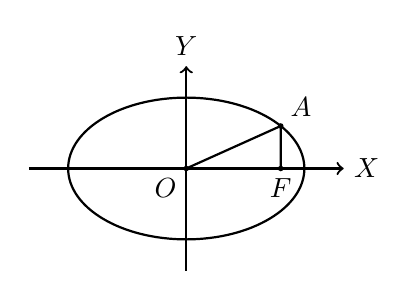
\begin{tikzpicture}[scale=1]
  \draw[thick,->] (-2,0) -- (2,0) node[right] {$X$};
  \draw[thick,->] (0,-1.3) -- (0,1.3) node[above] {$Y$};
  \draw[thick] (0,0) ellipse (1.5 and 0.9);
  \coordinate (O) at (0,0);
  \coordinate (F) at (1.2,0);
  \coordinate (A) at (1.2,0.54);
  \draw[thick] (O) -- (A) -- (F);
  \fill (O) circle (1pt) node[below left] {$O$};
  \fill (F) circle (1pt) node[below] {$F$};
  \fill (A) circle (1pt) node[above right] {$A$};
\end{tikzpicture}
